 \documentclass[10pt,a4paper]{article}
\usepackage[utf8x]{inputenc}
\usepackage{ucs}
\usepackage{amsmath}
\usepackage{amsfonts}
\usepackage{amssymb}
\usepackage{a4wide}
\usepackage{comment}
\usepackage[pdftex]{graphicx}
\usepackage{epstopdf}
\newcommand{\cmd}[1]{\texttt{#1}}
\newcommand{\remove}{}
\newcommand{\dir}[1]{\textsf{#1}}
\newcommand{\pop}{Depiler\xspace}
\newcommand{\push}{Empiler\xspace}
\newcommand{\tete}{LireTete}
\newcommand{\sommet}{LireSommet}
\newcommand{\empt}{EstVide}
\newcommand{\enqueue}{Enfiler\xspace}
\newcommand{\dequeue}{Defiler\xspace}
\newcommand{\get}{\ensuremath{\leftarrow\ }}

\usepackage[textsize=small, textwidth=2cm, color=yellow]{todonotes}

\excludecomment{solution}
\includecomment{solution}

\title{IF111 - Algorithmes et structures de données-TD5 :\\ Algorithmes de plus courts chemins}
\date{}
\author{\underline{Jonathan Narboni}, Rohan Fossé}
\date{\underline{\texttt{jonathan.narboni@labri.fr}}, \texttt{rfosse@labri.fr}}


\begin{document}
\maketitle

\section*{Exercice 1}
En utilisant l'algorithme de Djisktra, déterminez le plus court chemin entre le sommet \textbf{s} et \textbf{t}.

\begin{figure}[h!]
    \centering
    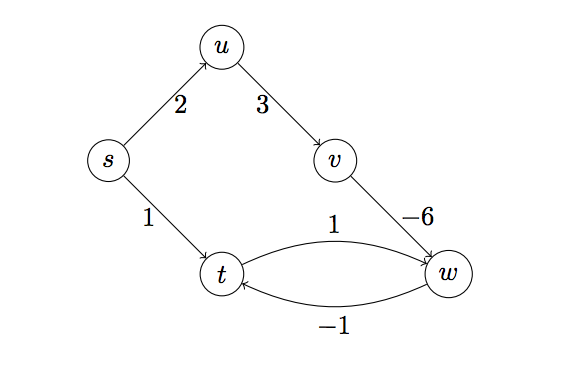
\includegraphics[scale=0.8]{DJ-1.png}
    \label{fig:my_label}
\end{figure}



\section*{Exercice 2}
En utilisant l'algorithme de Bellman-Ford, déterminez les plus courts chemins depuis le sommet 1.

\begin{figure}[h!]
    \centering
    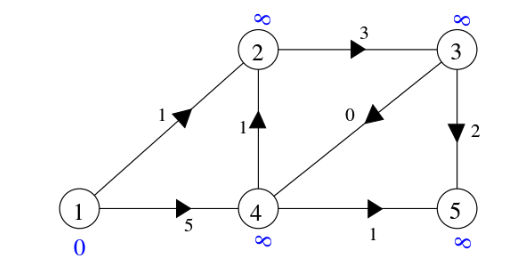
\includegraphics[scale=0.55]{BF-cours.png}
    \label{fig:my_label}
\end{figure}

\newpage 
\section*{Exercice 3}
Appliquez l'algorithme de Bellman-Ford sur le graphe suivant pour déterminer le plus court chemin de \textbf{s} à \textbf{p}.

\begin{figure}[h!]
    \centering
    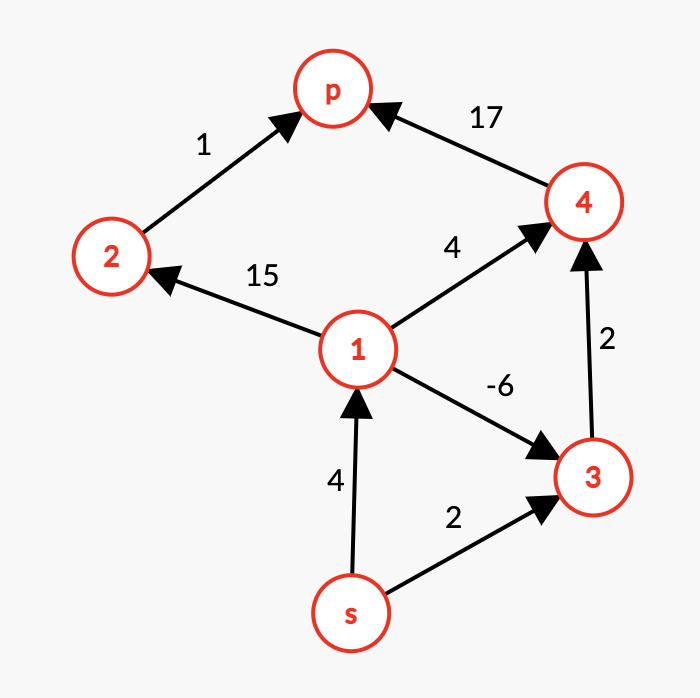
\includegraphics[scale=0.55]{BF-1.png}
\end{figure}

\section*{Exercice 4}
En utilisant l'algorithme de Bellman-Ford, déterminez les plus courts chemins depuis le sommet \textbf{s}.
\begin{figure}[h!]
    \centering
    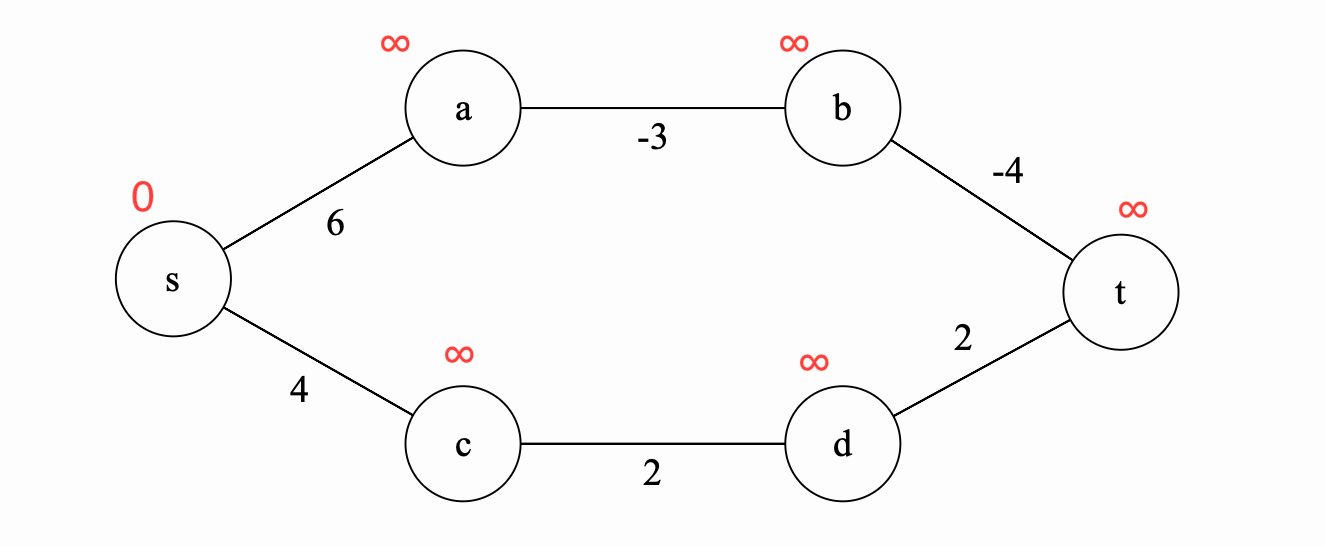
\includegraphics[scale=0.35]{BF-2.png}
    \label{fig:my_label}
\end{figure}

\end{document}


